\documentclass[a4paper,10pt] {article}
\usepackage[top=3cm,left=3cm,right=2cm,bottom=2cm]{geometry} % definir margens da página %
\usepackage[utf8]{inputenc} % suporte a acentos %
\usepackage{graphicx} % incluir figuras %
\usepackage[portuguese]{babel}

\begin{document}

\begin {center}
UNIVERSIDADE FEDERAL DO RIO GRANDE DO SUL

Programa de Pós-Graduação em Computação - PPGC

Concepção de Circuitos VLSI - CMP115

Professor Sergio Bampi

Aluno: Daniel Munari Palomino 

\vspace{7mm}
\textbf{ TRABALHO PRÁTICO 2 - \textit{BUFFER} }
\vspace{7mm}

\end{center}

\section{Objetivo}
Projetar um \textit{layout} de um \textit{buffer} \textit{tappered} de $N$ estágios e realizar a verificação, extração de capacitâncias parasitas a partir do \textit{layout}. Além disso, realizar a caracterização elétrica do \textit{buffer} gerar os seguintes resultados:

\begin{itemize}
\item Margens de ruído High e Low, obtidas a partir da função de transferência DC.
\item Valores dos tempos de resposta para o inversor projetado ($Tp_{hl}$, $Tp_{lh}$, $T_{rise}$ e $T_{fall}$).
\item Medir a potência consumida pelo inversor projetado à uma frequencia de chaveamento de 200MHz.
\item Calcular a energia média consumida por um par de transições L-$>$H e H-$>$L na saída do \textit{buffer}.

\end{itemize}

\section{Projeto e Dimensionamento do \textit{Buffer}}
O dimensionamento do \textit{buffer} foi realizado com o objetivo de minimizar o atraso. Todo o projeto foi realizado utilizando como base o inversor projetado no trabalho 1. A figura \ref{fig:inv} apresenta o \textit{layout} do inversor utilizado como base.

\begin{figure}[h]
	\centering
	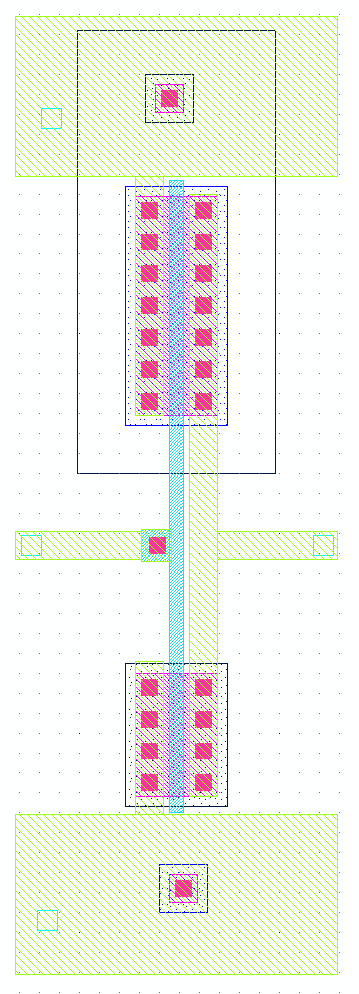
\includegraphics[scale=0.3]{layout_inversor.png}
	\caption{Layout do inversor INV\_1X}
	\label{fig:inv}
\end{figure}

Primeiramente foi calculado o valor da capacitância de entrada Cgin, com base nas dimensões do inversor INV\_1X.

\vspace{2mm}
$Cgin=(Wp+Wn).L.Cox$

$Cgin=(5,5$$\mu$$m+3,1$$\mu$$m).0,35$$\mu$$m.4,54fF$

$Cgin=13,67fF$

\vspace{2mm}

Em seguida, foi realizado o cálculo do Fan-Out Efetivo.
\vspace{2mm}

$F=CL/Cgin$

$F=1pF/13,67fF$

$F=73,15$
\vspace{2mm}

Com base no Fan-Out efetivo (F) foi então realizado o dimensionamento do \textit{buffer}. O número de estágios foi definido visando minimizar o atraso. A tabela \ref{tab:table1} apresenta o cálculo realizado para obtenção do número de estágios que foi utilizado no \textit{buffer}. As equações utilizadas abaixo são referentes ao $f$ (fator de sizing entre os estágios) e $tp$ que é o atraso do \textit{buffer}. Neste cálculo o valor de $tp0$ foi abstraído, pois é um valor constante e o valor de $\gamma$ utilizado foi igual a 1.

\begin{table}[h]
	\centering
	\caption{Cálculo do número de estágios para o \textit{buffer}.}
	\begin{tabular}{c|c|c}
		\hline
		$N$ & $f=\sqrt[N]{F}$ & $tp=N.tp0.(1+f/$$\gamma$$)$\\
		\hline
		1 & 73,15 & 74,15 $tp0$ \\
		2 & 8,55  & 19,1 $tp0$ \\
		\textbf{3} & \textbf{4,12}  & \textbf {15,36 $tp0$} \\
		4 & 2,92  & 15,68 $tp0$ \\
 		\hline
	\end{tabular}
	\label{tab:table1}
\end{table}

Considerando os resultados apresentados na tabela \ref{tab:table1}, o \textit{buffer} foi projetado com 3 estágios e com um fator de \textit{sizing} $f$ igual a 4,12. Desse modo, as dimensões dos inversores que compões o \textit{buffer} foram as seguintes:

\begin{itemize}
\item INV\_1: $Wp=5,5$$\mu$m e $Wn=3,1$$\mu$m
\item INV\_2: $Wp=22,0$$\mu$m e $Wn=12,4$$\mu$m
\item INV\_3: $Wp=88,0$$\mu$m e $Wn=49,6$$\mu$m
\end{itemize}

A figura \ref{fig:buffer} apresenta o \textit{layout} do \textit{buffer} considerando os cálculos apresentados anteriormente. A técnica de \textit{foldding} foi utilizada para possibilitar o \textit{layout} do \textit{buffer} no espaço determinado na especificação do trabalho (altura da célula, 20$\mu$m).

\begin{figure} [h]
	\centering
	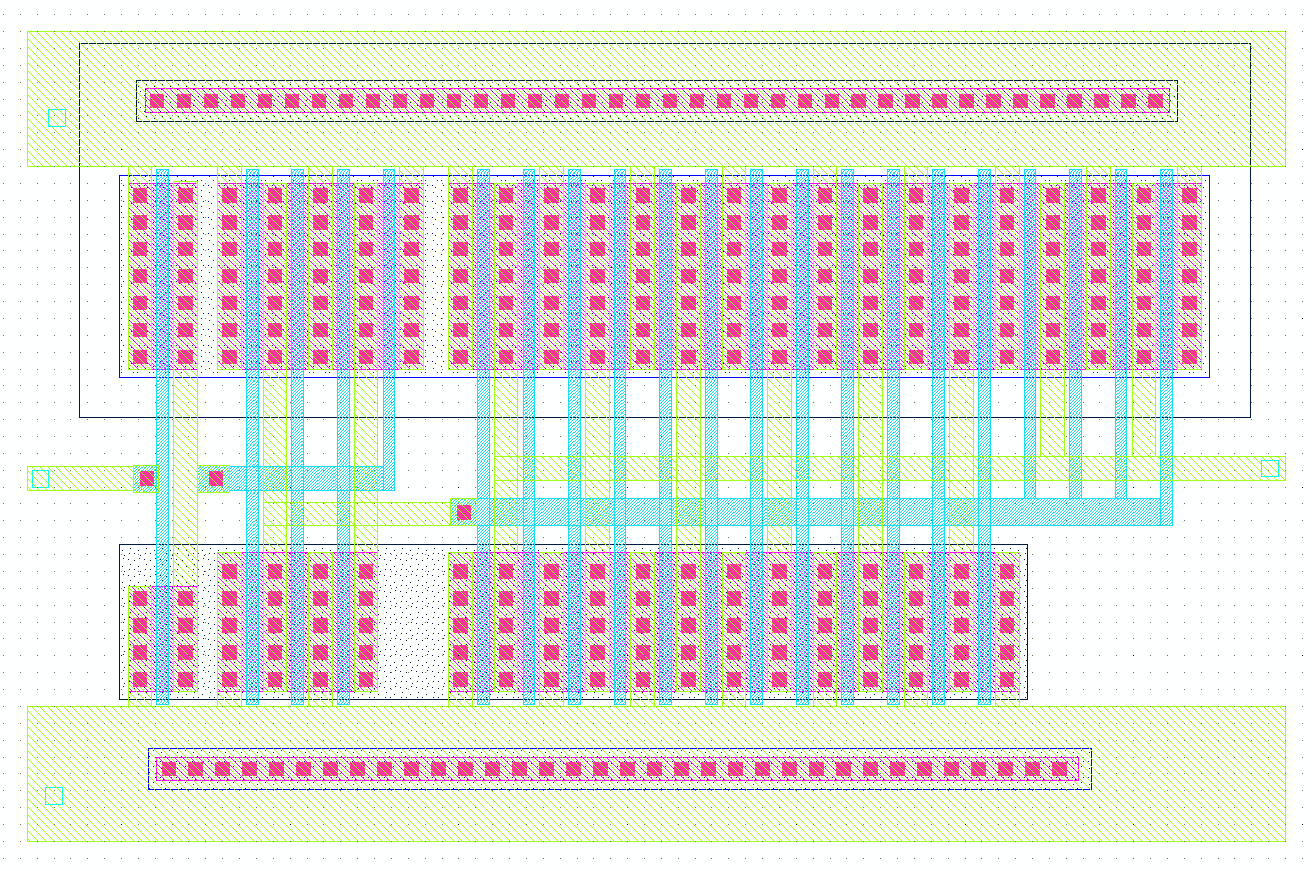
\includegraphics[scale=0.25]{layout_buffer.png}
	\caption{Layout do \textit{buffer} projetado}
	\label{fig:buffer}
\end{figure}

\section{Verificações}
\label{sec:veri}
A primeira verficação realizada sobre o projeto do \textit{layout} do \textit{buffer} foi a verficação DRC. A figura \ref{fig:drc} apresenta a saída do software para a verficação DRC. É possível observar que nenhum erro foi encontrado.

\begin{figure} [h]
	\centering
	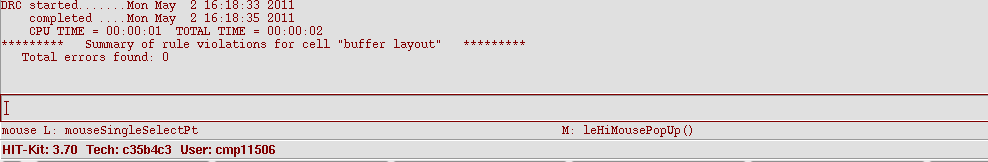
\includegraphics[scale=0.4]{DRC_buffer.png}
	\caption{Resultado verficação DRC.}
	\label{fig:drc}
\end{figure}

O esquemático do \textit{buffer} também foi construído, afim de realizar a verificação LVS (\textit{layout versus squematic}). A figura \ref{fig:esquematico} apresenta o esquemático referente ao \textit{buffer} projetado e a figura \ref{fig:lvs} apresenta o resultado da verificação LVS.

\begin{figure} [h]
	\centering
	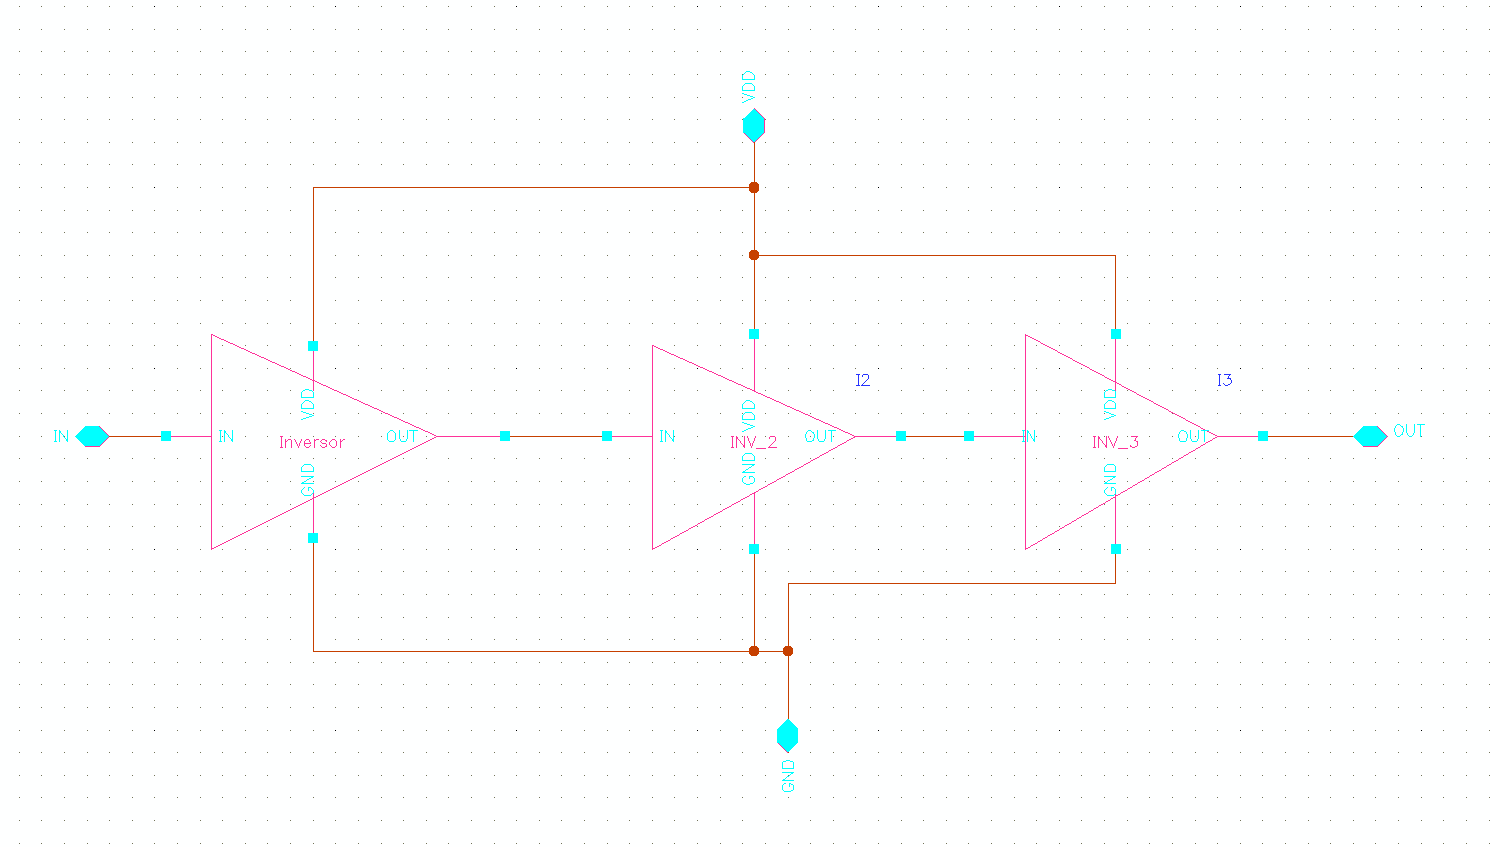
\includegraphics[scale=0.3]{esquematico_buffer.png}
	\caption{Esquemático do \textit{buffer} projetado.}
	\label{fig:esquematico}
\end{figure}

\begin{figure} [h]
	\centering
	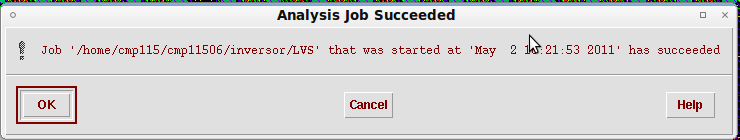
\includegraphics[scale=0.6]{LVS_buffer.png}
	\caption{Resultado da verificação LVS.}
	\label{fig:lvs}
\end{figure}

A extração das capacitâncias parasitas também foi realizada. O \textit{layout} com as capacitância parasitas extraídas foi utilizado para realizar a caracterização elétrica do \textit{buffer} projetado, que será apresentada na próxima seção. A figura \ref{fig:extraido} apresenta o \textit{layout} do \textit{buffer} com as capacitâncias parasitas extraídas.

\begin{figure} [h]
	\centering
	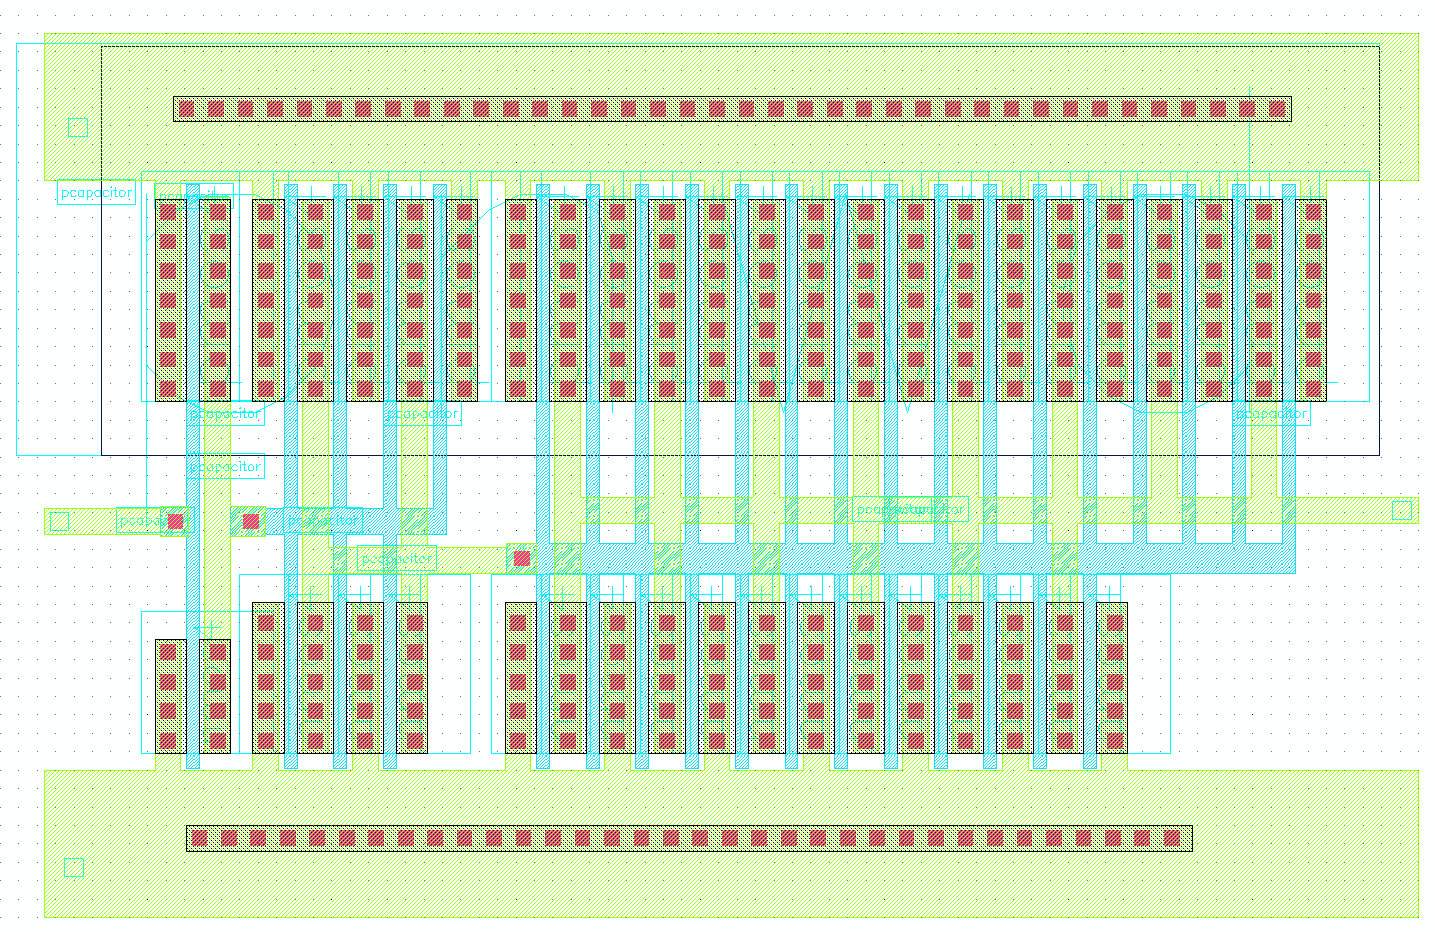
\includegraphics[scale=0.2]{extraido_buffer.png}
	\caption{Layout do \textit{buffer} projetado com as capacitâncias parasitas extraídas.}
	\label{fig:extraido}
\end{figure}

\section{Caracterização Elétrica}
\label{sec:caracterizacao}
O modelo de simulação utilizado está representado na figura \ref{fig:teste}. A fonte vdc na entrada foi utilizada para obter a curva de transferência DC enquanto que a fonte vpulse foi utilizada para realizar a ánalise transiente. A carga utilizada na saída é de $1pF$, como descrito na especificação.

\begin{figure} [h]
	\centering
	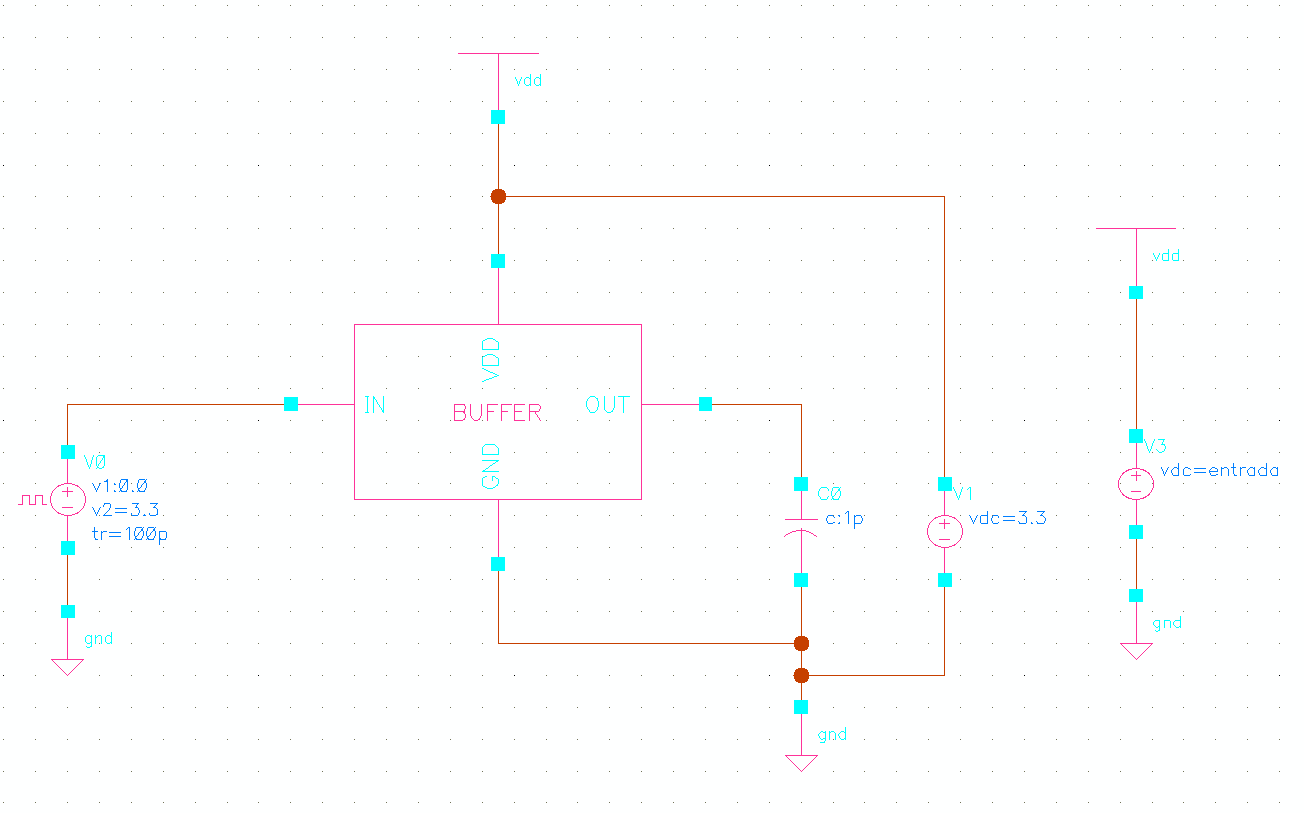
\includegraphics[scale=0.15]{teste_buffer.png}
	\caption{Modelo de simulação utilizado para realizar a caracterização elétrica do \textit{buffer}.}
	\label{fig:teste}
\end{figure}

Primeiramente foi gerada a função de transferência DC para o cálculo das margens de ruído High e Low. A figura \ref{fig:dc} apresenta a curva que representa função de transferência DC onde os pontos marcados são referentes aos limites das margens de ruído.

\begin{figure} [h]
	\centering
	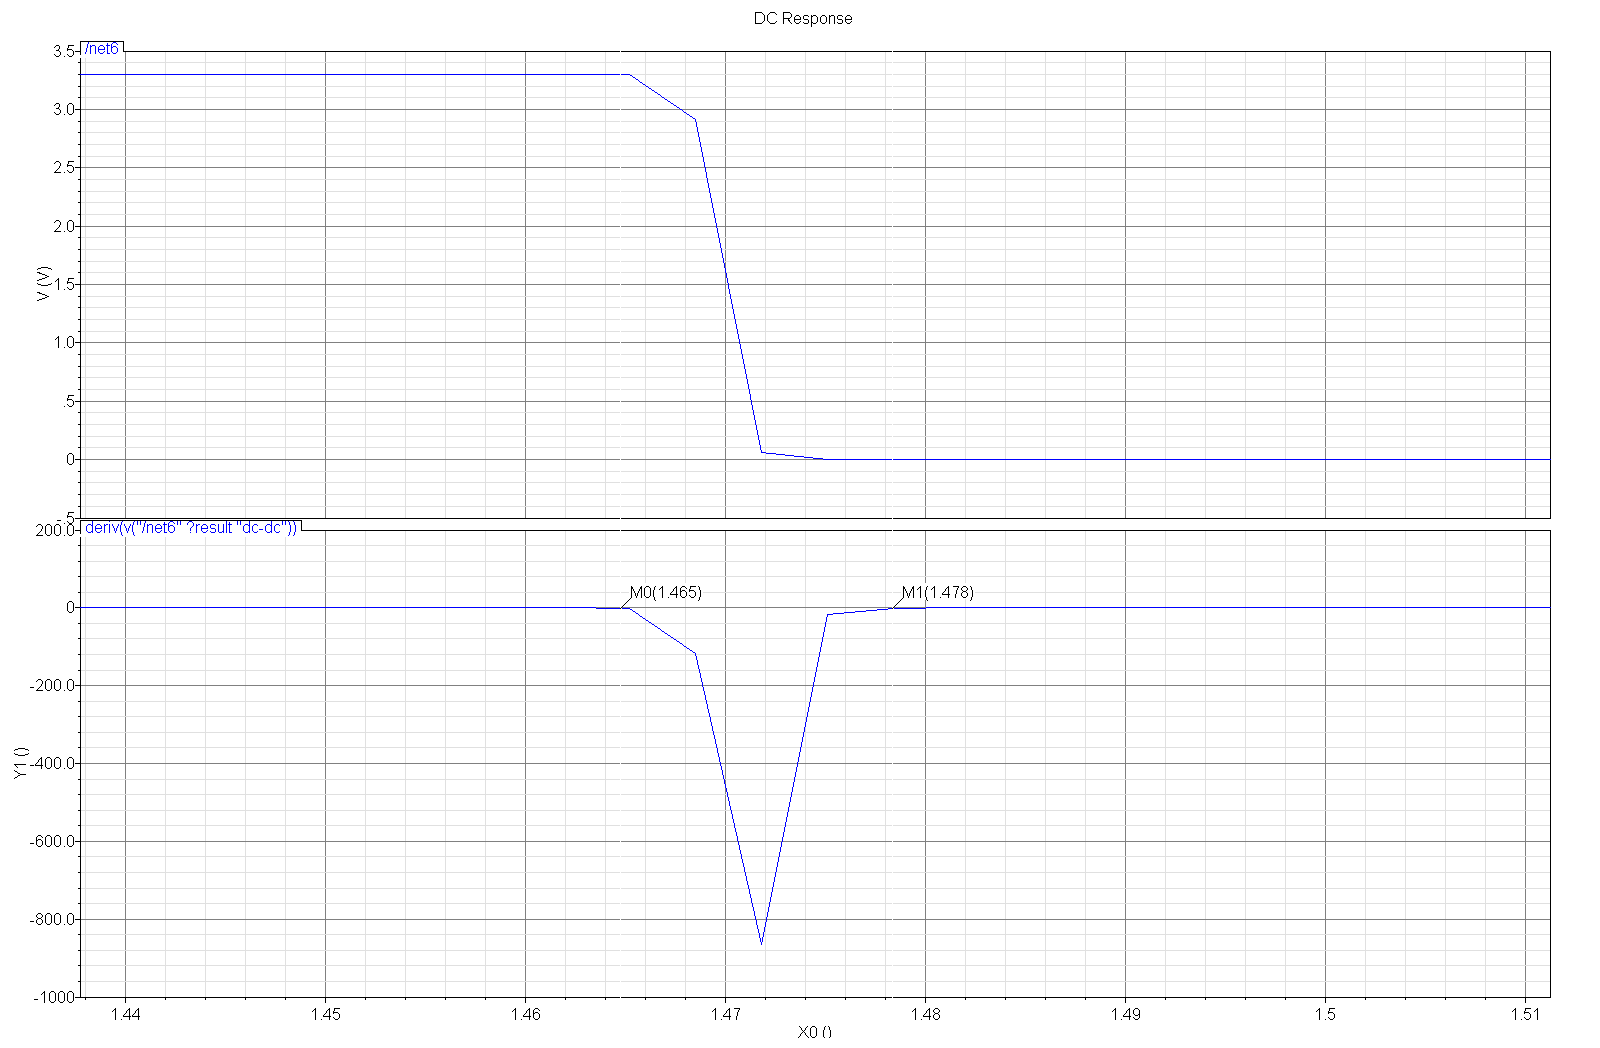
\includegraphics[scale=0.1]{DC_Buffer.png}
	\caption{Curva de transferência DC.}
	\label{fig:dc}
\end{figure}

Desse modo, a margem de ruído Low é 0V à 1.465V e a margem de ruiído High é 1.478V à 3.3V.

Considerando a ánalise transiente realizada, quatro tempos de resposta foram obtidos: (1)$Tp_{hl}$ (tempo de high low), (2$)Tp_{lh}$ (tempo de low high), (3)$T_{rise}$ (tempo de subida) e (4)$T_{fall}$ (tempo de descida). As figuras \ref{fig:hl}, \ref{fig:lh}, \ref{fig:rise} e \ref{fig:fall} mostram como esses tempos foram obtidos.

\begin{figure} [h]
	\begin{minipage} [b] {0.48 \linewidth}
		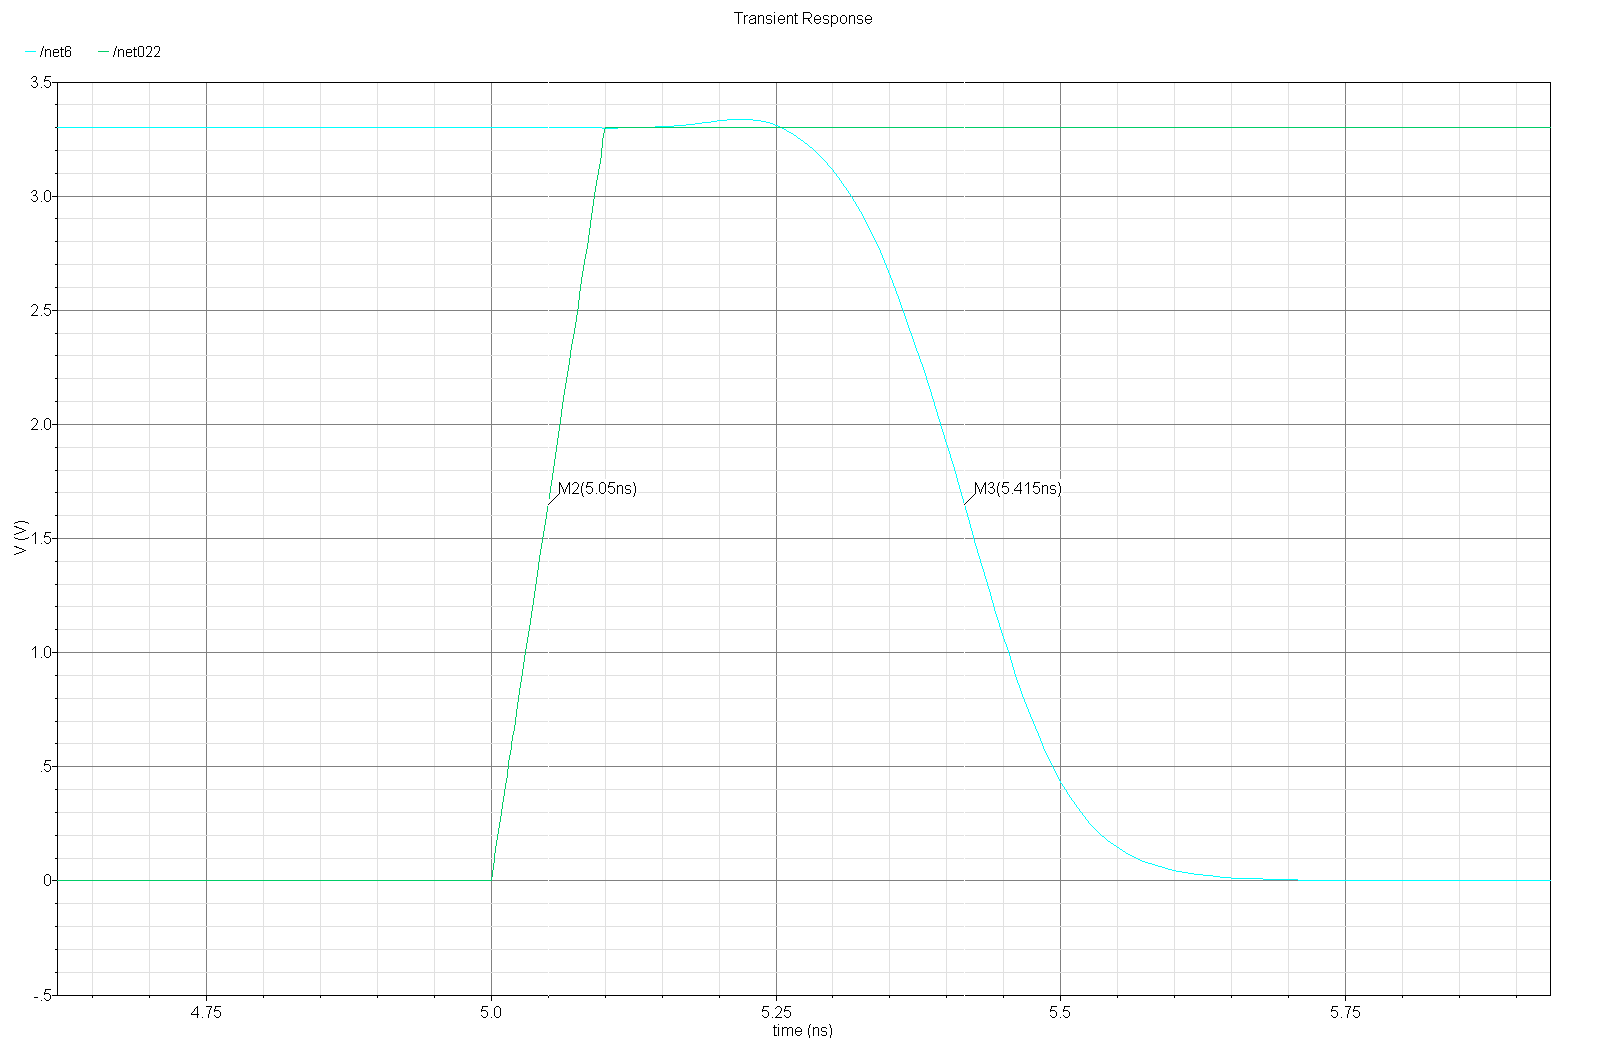
\includegraphics[scale=0.1]{Trans_HL.png}
		\centering
		\caption{Curva de tempo High Low.}
		\label{fig:hl}
	\end{minipage}
	\begin{minipage} [b] {0.48 \linewidth}
		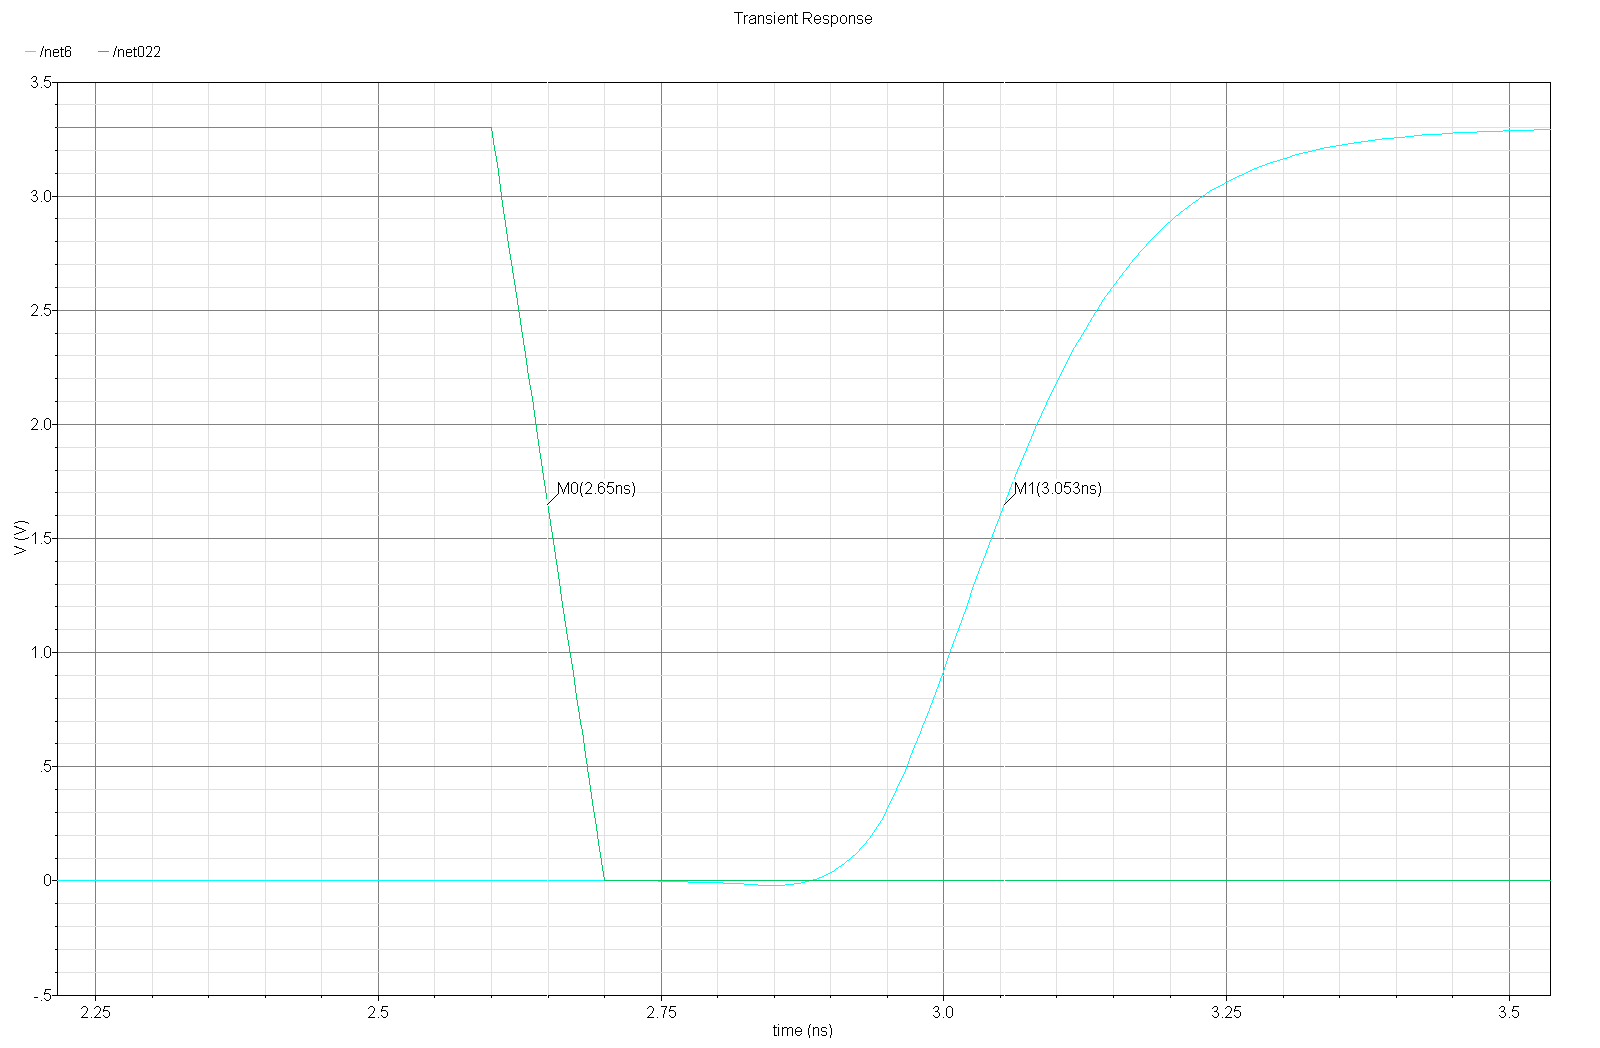
\includegraphics[scale=0.1]{Trans_LH.png}
		\centering
		\caption{Curva de tempo Low High.}
		\label{fig:lh}
	\end{minipage}
\end{figure}

\begin{figure} [h]
	\begin{minipage} [b] {0.48 \linewidth}
		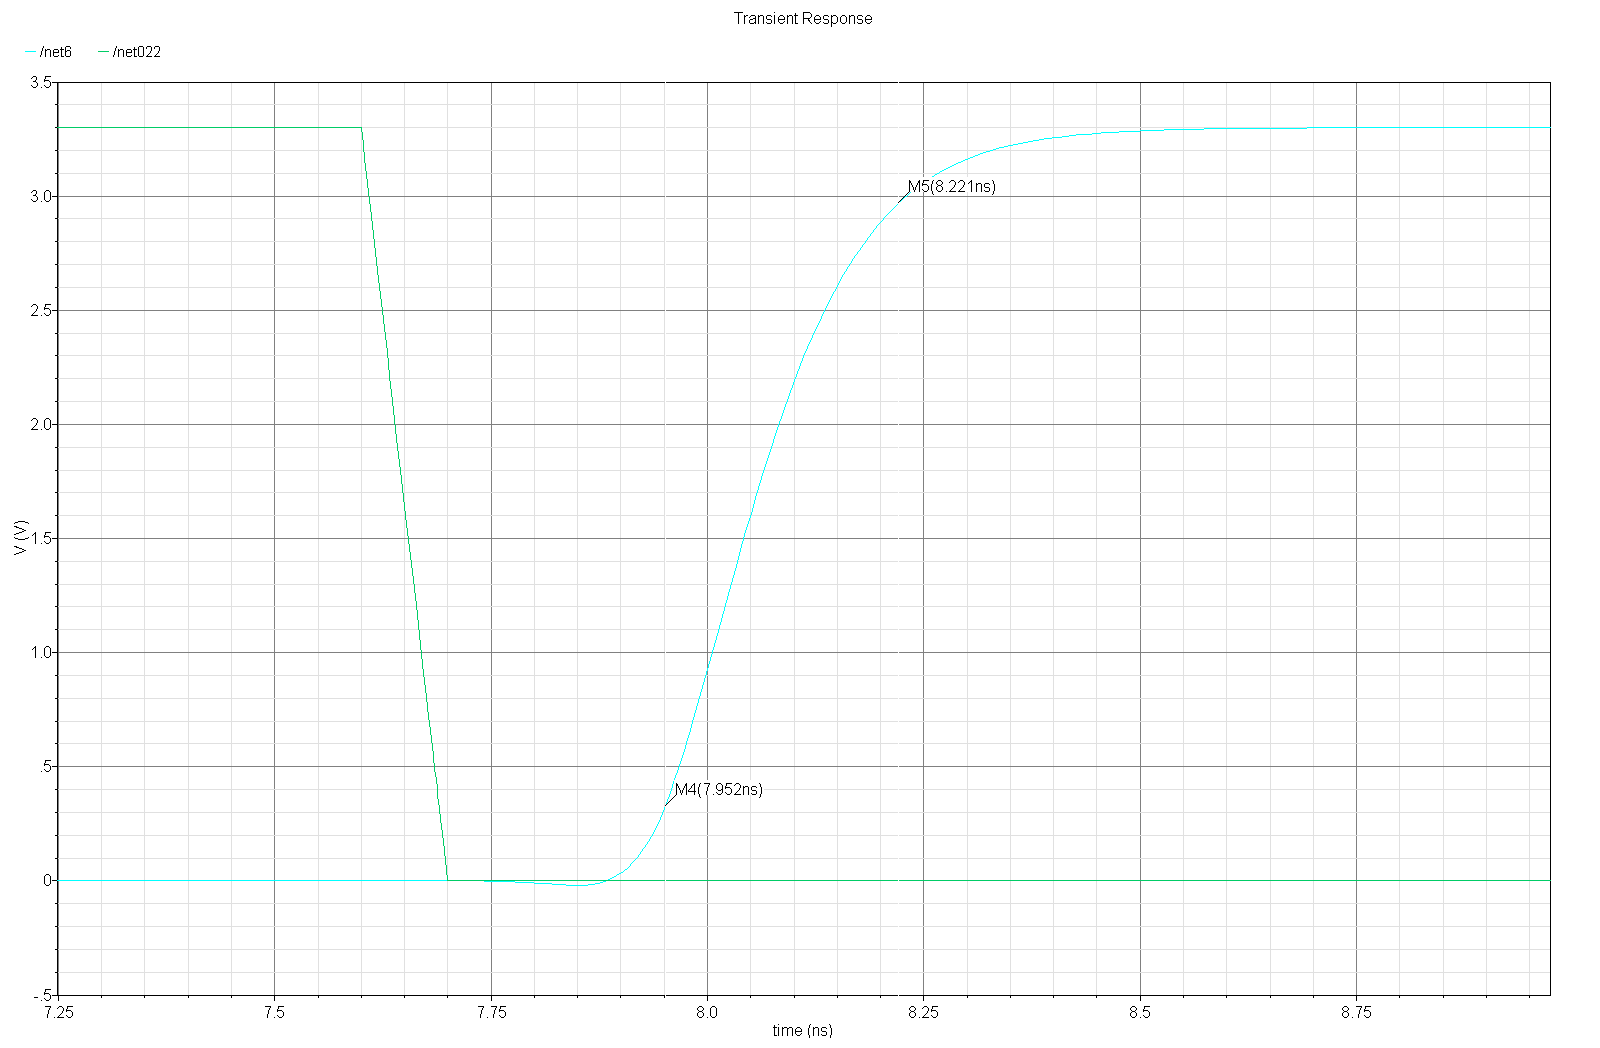
\includegraphics[scale=0.1]{Trans_rise.png}
		\centering
		\caption{Curva de tempo de subida.}
		\label{fig:rise}
	\end{minipage}
	\begin{minipage} [b] {0.48 \linewidth}
		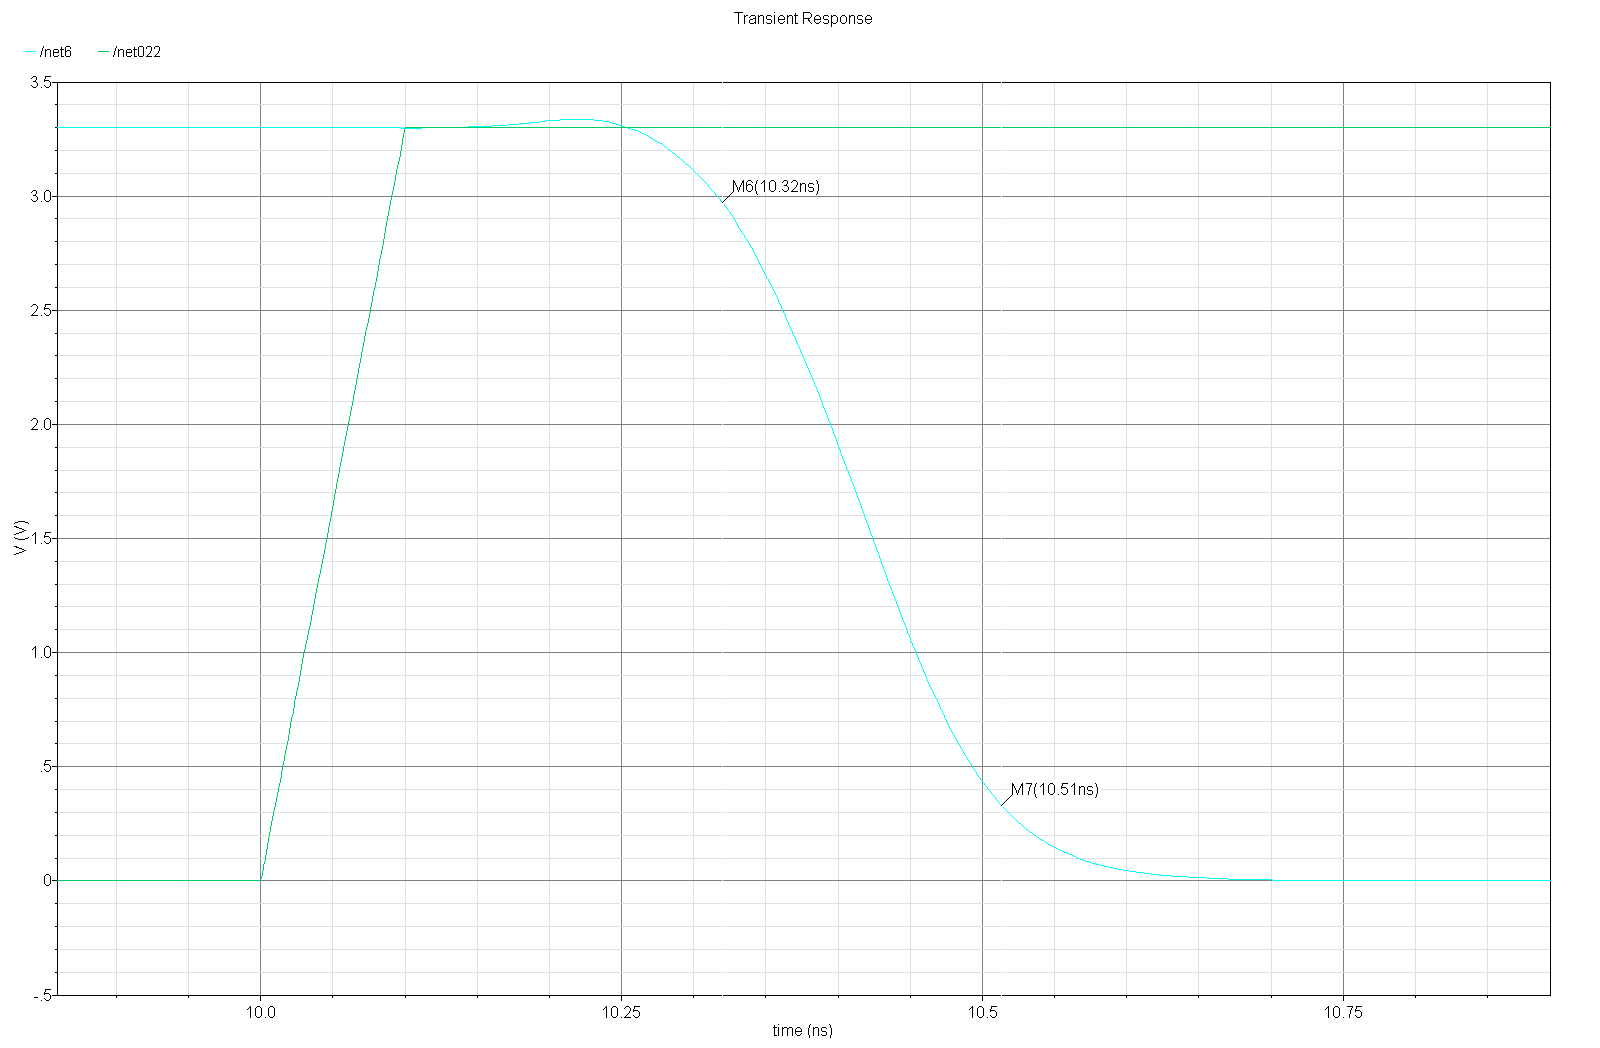
\includegraphics[scale=0.1]{Trans_fall.png}
		\centering
		\caption{Curva de tempo de descida.}
		\label{fig:fall}
	\end{minipage}
\end{figure}

Com base nas curvas apresentadas acima, os tempos de resposta para o \textit{buffer} projetado foram os seguintes:

\begin{itemize}
\item $Tp_{hl}=M3-M2=5,415ns-5,050ns=0.365ns$
\item $Tp_{lh}=M1-M0=3,053ns-2,650ns=0.403ns$
\item $T_{rise}=M5-M4=8,221ns-7,952ns=0,269ns$
\item $T_{fall}=M7-M6=10,51ns-10,32ns=0,19ns$
\end{itemize}

O passo seguinte foi realizar a medição da potência consumida pelo \textit{buffer} projetado. O modelo de simulação mostrado na figura \ref{fig:teste} também foi utilizado nesta etapa. A frequência de chaveamento utilizada foi de 200MHz. A figura \ref{fig:corrente} mostar a curva que representa a corrente de alimentação utilizada no cálculo da potência.

\begin{figure} [h]
	\centering
	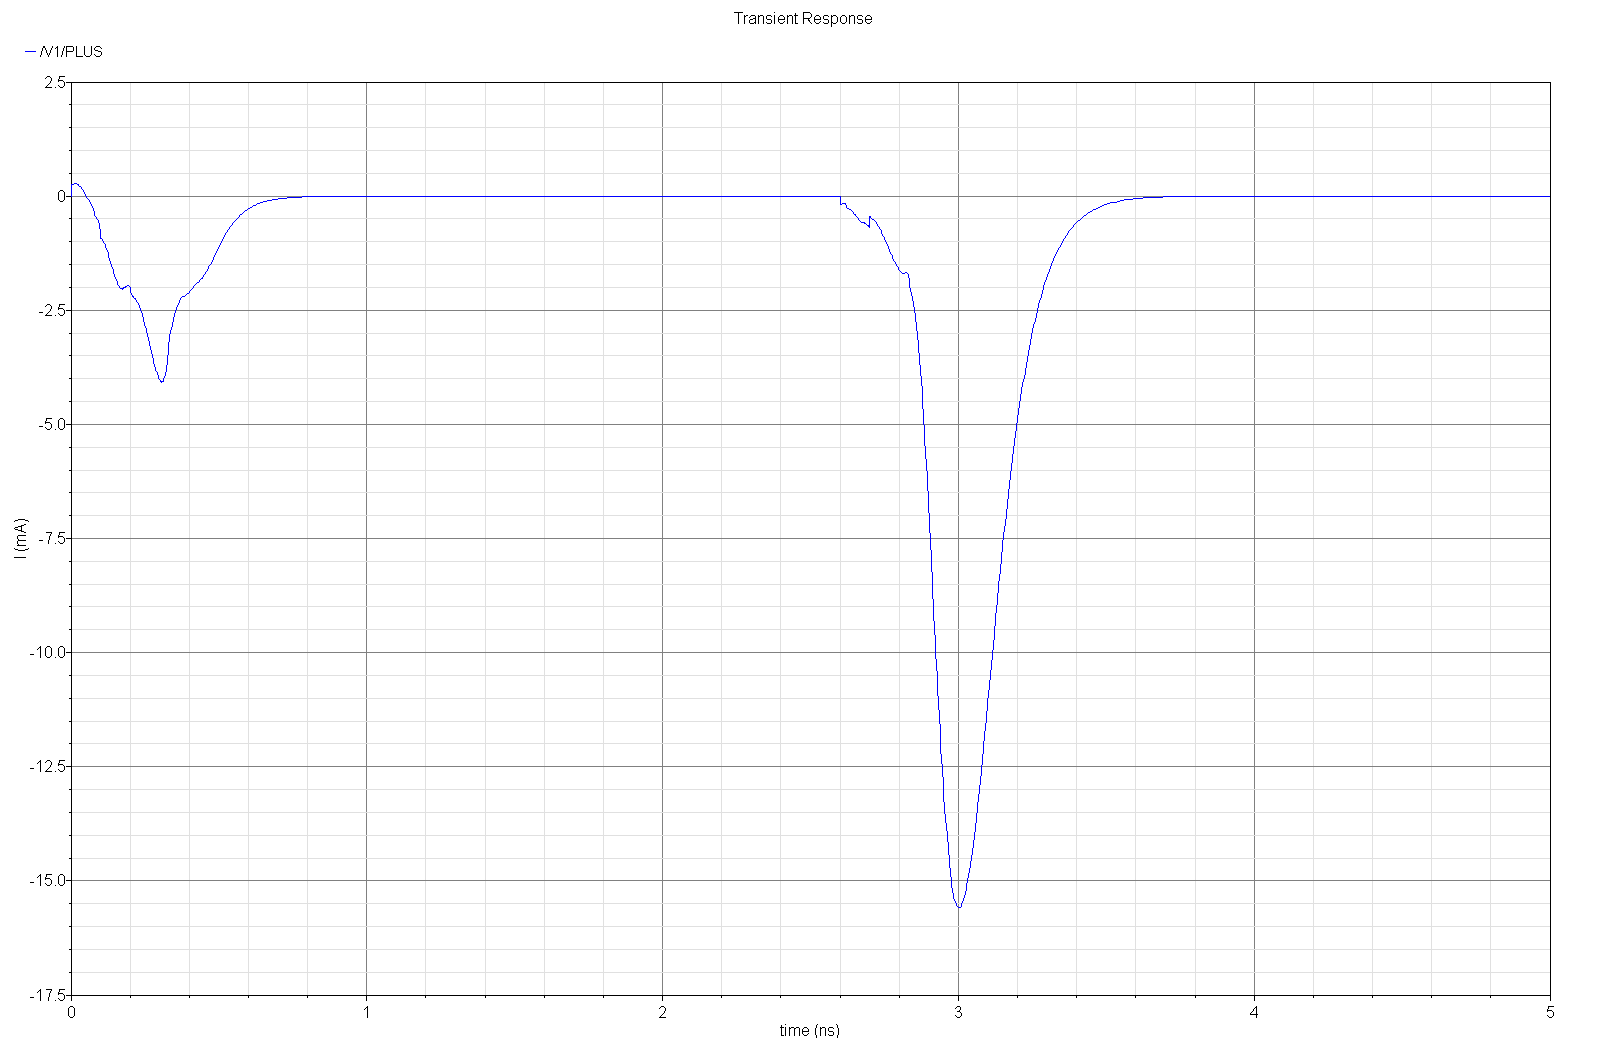
\includegraphics[scale=0.1]{Corrente.png}
	\caption{Corrente de entrada.}
	\label{fig:corrente}
\end{figure}

A potência consumida pelo inversor foi de 3,511mW. Sendo assim, a energia consumida por uma par de transições L-$>$H e H-$>$L na saída do inversor foi de 17,6pJ.

\section{Referências}
\begin{enumerate}
\item Rabaey, J., Chandrakasan, \textordfeminine,Nikolic, B. - "Digital Integrated Circuits - A Design Perspective". Prentice Hall, 2\textordfeminine Edição. ISBN 0-13178609-1.
\item AMS 0.35$\mu$m CMOS C35 Design Rules revisão 2.0, 2003.
\end{enumerate}

\end{document}
